
\documentclass[a4paper,11pt]{article}
\usepackage[a4paper, margin=8em]{geometry}

% usa i pacchetti per la scrittura in italiano
\usepackage[french,italian]{babel}
\usepackage[T1]{fontenc}
\usepackage[utf8]{inputenc}
\frenchspacing 

% usa i pacchetti per la formattazione matematica
\usepackage{amsmath, amssymb, amsthm, amsfonts}

% usa altri pacchetti
\usepackage{gensymb}
\usepackage{hyperref}
\usepackage{standalone}

% imposta il titolo
\title{Appunti Comunicazioni Numeriche}
\author{Luca Seggiani}
\date{2026}

% imposta lo stile
% usa helvetica
\usepackage[scaled]{helvet}
% usa palatino
\usepackage{palatino}
% usa un font monospazio guardabile
\usepackage{lmodern}

\renewcommand{\rmdefault}{ppl}
\renewcommand{\sfdefault}{phv}
\renewcommand{\ttdefault}{lmtt}

% disponi il titolo
\makeatletter
\renewcommand{\maketitle} {
	\begin{center} 
		\begin{minipage}[t]{.8\textwidth}
			\textsf{\huge\bfseries \@title} 
		\end{minipage}%
		\begin{minipage}[t]{.2\textwidth}
			\raggedleft \vspace{-1.65em}
			\textsf{\small \@author} \vfill
			\textsf{\small \@date}
		\end{minipage}
		\par
	\end{center}

	\thispagestyle{empty}
	\pagestyle{fancy}
}
\makeatother

% disponi teoremi
\usepackage{tcolorbox}
\newtcolorbox[auto counter, number within=section]{theorem}[2][]{%
	colback=blue!10, 
	colframe=blue!40!black, 
	sharp corners=northwest,
	fonttitle=\sffamily\bfseries, 
	title=~\thetcbcounter: #2, 
	#1
}

% disponi definizioni
\newtcolorbox[auto counter, number within=section]{definition}[2][]{%
	colback=red!10,
	colframe=red!40!black,
	sharp corners=northwest,
	fonttitle=\sffamily\bfseries,
	title=~\thetcbcounter: #2,
	#1
}

% U.D.M
\newcommand{\amp}{\ensuremath{\mathrm{A}}}
\newcommand{\volt}{\ensuremath{\mathrm{V}}}
\newcommand{\meter}{\ensuremath{\mathrm{m}}}
\newcommand{\second}{\ensuremath{\mathrm{s}}}
\newcommand{\farad}{\ensuremath{\mathrm{F}}}
\newcommand{\henry}{\ensuremath{\mathrm{H}}}
\newcommand{\siemens}{\ensuremath{\mathrm{S}}}

% circuiti
\usepackage{circuitikz}
\usetikzlibrary{babel}

% disegni
\usepackage{pgfplots}
\pgfplotsset{width=10cm,compat=1.9}

% disponi codice
\usepackage{listings}
\usepackage[table]{xcolor}

\lstdefinestyle{codestyle}{
		backgroundcolor=\color{black!5}, 
		commentstyle=\color{codegreen},
		keywordstyle=\bfseries\color{magenta},
		numberstyle=\sffamily\tiny\color{black!60},
		stringstyle=\color{green!50!black},
		basicstyle=\ttfamily\footnotesize,
		breakatwhitespace=false,         
		breaklines=true,                 
		captionpos=b,                    
		keepspaces=true,                 
		numbers=left,                    
		numbersep=5pt,                  
		showspaces=false,                
		showstringspaces=false,
		showtabs=false,                  
		tabsize=2
}

\lstdefinestyle{shellstyle}{
		backgroundcolor=\color{black!5}, 
		basicstyle=\ttfamily\footnotesize\color{black}, 
		commentstyle=\color{black}, 
		keywordstyle=\color{black},
		numberstyle=\color{black!5},
		stringstyle=\color{black}, 
		showspaces=false,
		showstringspaces=false, 
		showtabs=false, 
		tabsize=2, 
		numbers=none, 
		breaklines=true
}

\lstdefinelanguage{javascript}{
	keywords={typeof, new, true, false, catch, function, return, null, catch, switch, var, if, in, while, do, else, case, break},
	keywordstyle=\color{blue}\bfseries,
	ndkeywords={class, export, boolean, throw, implements, import, this},
	ndkeywordstyle=\color{darkgray}\bfseries,
	identifierstyle=\color{black},
	sensitive=false,
	comment=[l]{//},
	morecomment=[s]{/*}{*/},
	commentstyle=\color{purple}\ttfamily,
	stringstyle=\color{red}\ttfamily,
	morestring=[b]',
	morestring=[b]"
}

% disponi sezioni
\usepackage{titlesec}

\titleformat{\section}
	{\sffamily\Large\bfseries} 
	{\thesection}{1em}{} 
\titleformat{\subsection}
	{\sffamily\large\bfseries}   
	{\thesubsection}{1em}{} 
\titleformat{\subsubsection}
	{\sffamily\normalsize\bfseries} 
	{\thesubsubsection}{1em}{}

% disponi alberi
\usepackage{forest}

\forestset{
	rectstyle/.style={
		for tree={rectangle,draw,font=\large\sffamily}
	},
	roundstyle/.style={
		for tree={circle,draw,font=\large}
	}
}

% disponi algoritmi
\usepackage{algorithm}
\usepackage{algorithmic}
\makeatletter
\renewcommand{\ALG@name}{Algoritmo}
\makeatother

% disponi numeri di pagina
\usepackage{fancyhdr}
\fancyhf{} 
\fancyfoot[L]{\sffamily{\thepage}}

\makeatletter
\fancyhead[L]{\raisebox{1ex}[0pt][0pt]{\sffamily{\@title \ \@date}}} 
\fancyhead[R]{\raisebox{1ex}[0pt][0pt]{\sffamily{\@author}}}
\makeatother

\begin{document}
% sezione (data)
\section{Lezione del 29-05-26}

% stili pagina
\thispagestyle{empty}
\pagestyle{fancy}

% testo
Nella scorsa lezione abbiamo introdotto i sistemi in banda passante. Di questi avevamo detto che il segnale ricevuto era:
$$
r(t) = 2 r_{RF}(t) \cos(2 \pi f_0 t) = 2 S_{RF}(t) \cos(2 \pi f_0 t) + W(t)
$$
dove $W(t)$ era il rumore "demodulato". Da questo deriva che dopo il demodulatore, il segnale ricevuto:
$$
x(t) = \sum_k \sqrt{\beta} a_k g(t - k T_S) + n(t_T)
$$
dove $n'(k)$, il  rumore ricevuto, è dato da:
$$
n(k) = W_{RF}(t) 2 \cos(2 \pi f_0 t) \circledast g_R(t), \quad n(t) \in \mathcal{N}(0, N_0 E_{g_R})
$$
e dove ricordiamo che avevamo definito:
$$
W(t) = W_{RF}(t) 2 \cos(2 \pi f_0 t), \quad S_{W} \sim N_0
$$

\subsection{QAM}

I sistemi \textbf{QAM} (\textit{Quadrature Amplitude Modulation}) utilizzano delle mappe complesse, su 2 assi. Possiamo intedere queste mappe come 2 mappe PAM. Ad esempio, possiamo usare una 2-PAM reale con una 2-PAM immaginaria per ottenere una mappa a $16$ simboli:
\begin{center}
	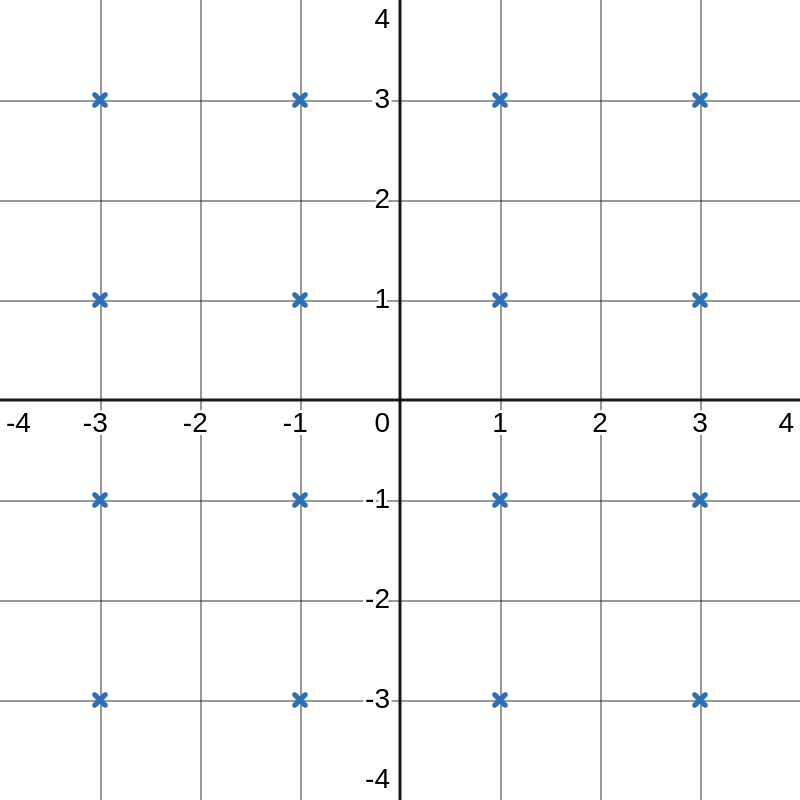
\includegraphics[scale=0.27]{../figures/qam16.png}
\end{center}
Nulla vieta di combinare PAM di ordine diverso. Una QAM con $N$ simboli viene detta $N$-PAM. 

\subsubsection{Mappatura di Gray}

Interroghiamoci su come realizzare una mappa di Gray per una QAM. Questa è una mappa che a parità di rumore minimizza la probabilità di errore: alternativamente vogliamo che simboli adiacenti differiscano fra di loro di un solo bit. 

Otteniamo una mappa di questo tipo, ad esempio un una 16-QAM, assegnando i primi, $2$ bit al primo quadrante, e quindi "ribaltando" la mappa in ogni quadrante per assicurare l'adiacenza di un solo bit al massimo. Quindi si indicizza ogni quadrante con i restanti $2$ bit.

\begin{center}
	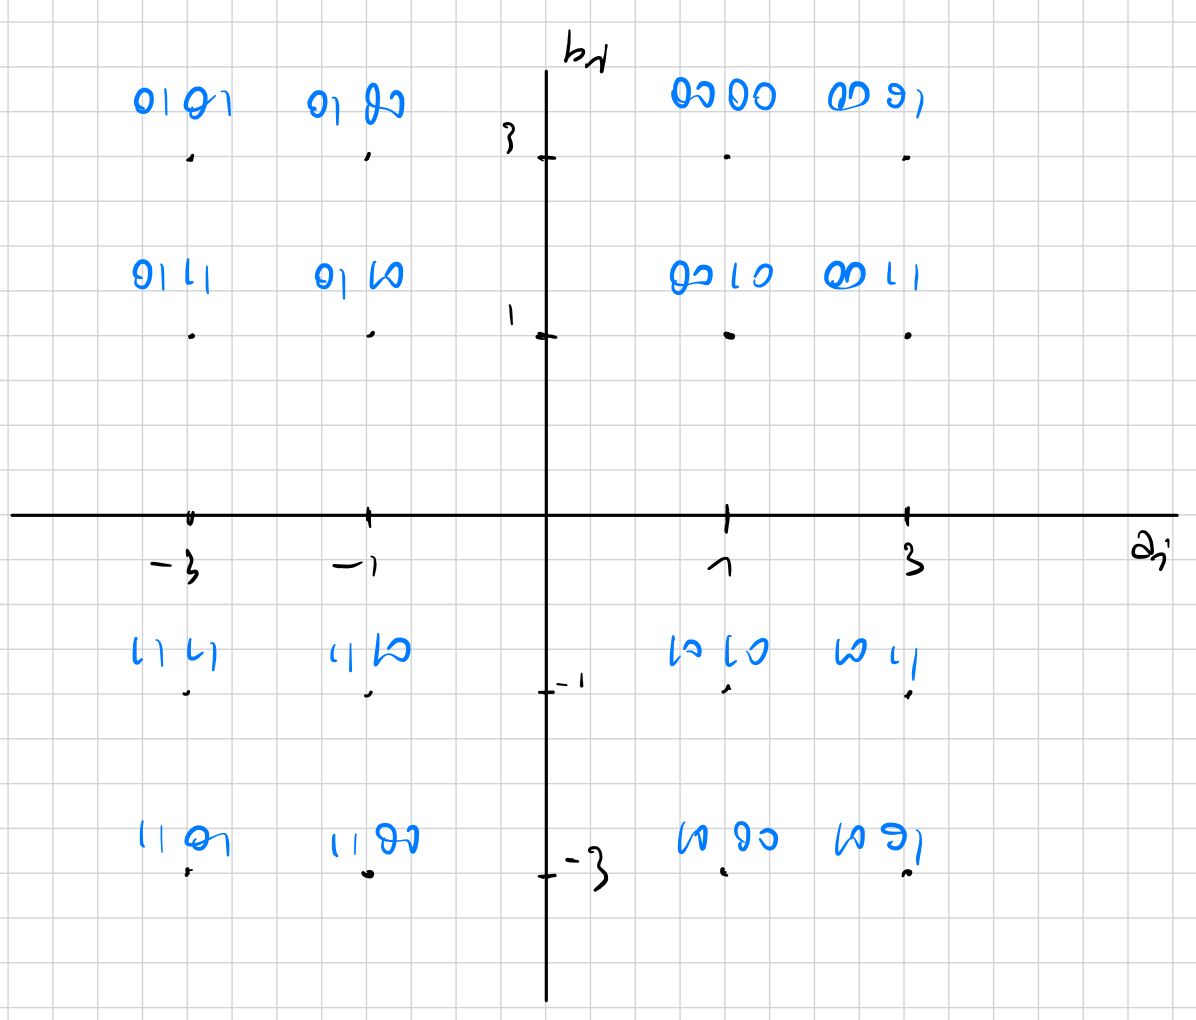
\includegraphics[scale=0.27]{../figures/qam16_note.png}
\end{center}

\subsection{Trasmettitore QAM}

Vediamo quindi l'implementazione del trasmettitore QAM. Questa si basa sul fatto che possiamo modulare il segnale in uscita da quelli che sono sostanzialmente due codificatori PAM, in maniera ortogonale (uno sul coseno e uno sul seno):
\begin{center}
	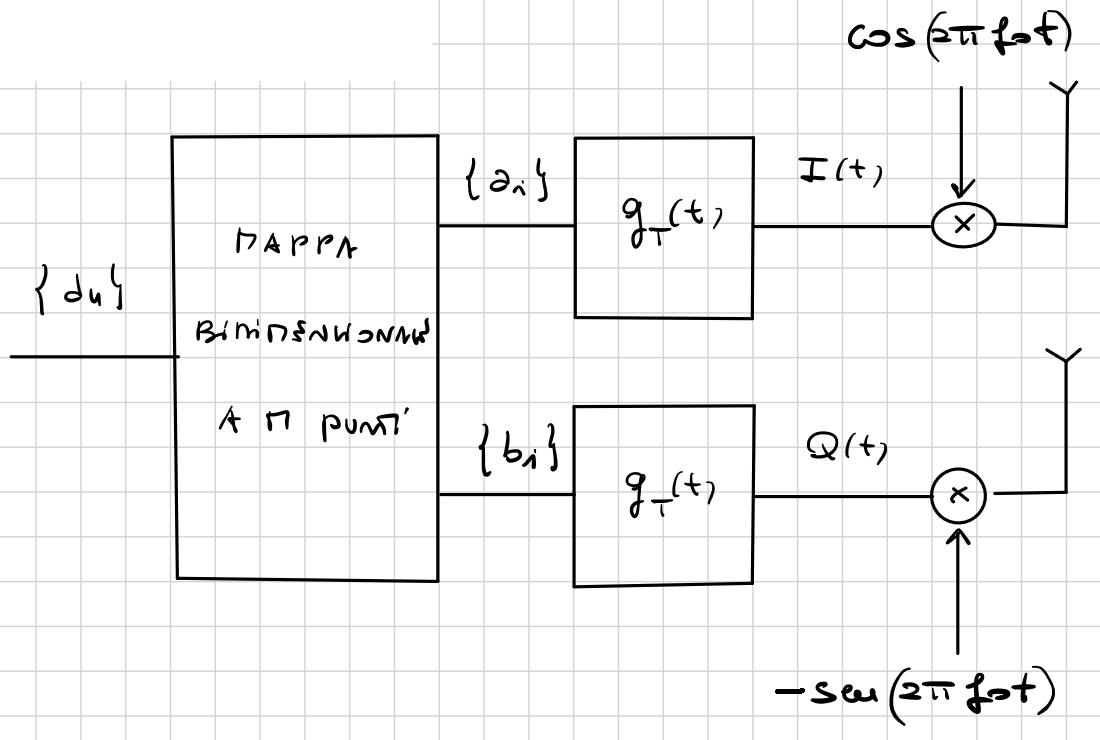
\includegraphics[scale=0.27]{../figures/qam_trans.png}
\end{center}

Per quanto ci riguarda nemmeno ci interessa sapere se i flussi di bit dal mappatore ($a_k$ e $b_k$) dipendono da un unico flusso di bit di codice, o sono indipendenti fra di loro. 

Ciò che ci interessa è il segnale che otteniamo sull'etere, dato dalla soma dei segnali alle 2 antenne (che dicevamo modulati in maniera ortogonale seno/coseno):
$$
S_{RF}(t) = I(t) \cos(2 \pi f_0 t) - Q(t) \sin(2 \pi f_0 t)
$$
dove vale che il filtro di trasmissione per i 2 flussi è il solito:
$$
\begin{cases}
	I(t) = \sum_i a_i g_T(t - i T_S) \\
	Q(t) = \sum_i b_i g_T(t - i T_S) \\
\end{cases}
$$

Il modo in cui possiamo rappresentare tale segnale è sul piano complesso, come:
$$
S_{RF}(t) = \mathrm{RE} \left\{ \tilde{S}(t) e^{j 2 \pi f_0 t} \right\}
$$
dove notiamo l'\textit{inviluppo complesso} $\tilde{S}$:
$$
\tilde{S}(t) = \sum_i c_i g_T(t - i T_S), \quad c_i = a_i + j b_i
$$

Matematicamente, questo sistema ammette un equivalente in banda base, equivalente al sistema PAM in banda base ma dove la mappa è complessa (derivata sopra).

\subsubsection{Considerazioni di potenza}

Continuiamo a trattare il trasmettitore, arrivando alle considerazioni di potenza. Abbiamo che la densità spettrale di potenza, dopo il modulatore, è:
$$
S_{RF}(f) = \frac{S_{\tilde{S}}(f - f_0) + S_{\tilde{S}}(f + f_0)}{4}
$$
dove la densità spettrale che da i 2 lobi è:
$$
S_{\tilde{S}} (f) = \frac{1}{T_S} \sigma_C^2 | G_T(f) |^2
$$
Calcoliamo la $\sigma_C^2$ (ovvero la varianza dell'inviluppo complesso, e quindi dei codici QAM che inviamo sul mezzo) come:
$$
\sigma_C^2 = E \{  | c_k |^2 \} = E \{ | a_k + j b_k |^2 \} = E \{ (a + j b_k) (a - j b_k) \} 
$$
$$
= E \{ a_k^2 \} - j E \{ a_k b_k \} + j E \{ b_k a_k \} + E \{ b_k^2 \}
= E \{ a_k^2 \} + E \{ b_k^2 \} = 2 \frac{M^2 - 1}{3}
$$

Abbiamo ottenuto tale risultato perché i termini al centro si cancellano e rimangono soltanto i valori quadratici medi dei 2 canali PAM. Quindi, visto che abbiamo scelto 2 PAM dello stesso ordine, otteniamo 2 volte la varianza di un singolo canale PAM.

\subsubsection{Considerazioni di banda}

Veniamo alla banda, che si può calcolare come:
$$
B_S = \frac{1 + \alpha}{T_S} = \frac{1 + \alpha}{\log_2 M^2} \frac{1}{T_d} = \frac{1 + \alpha}{r \log_2 M^2} \frac{1}{T_b}
$$
dove si prende $M^2$ come cardinalità dell'alfabeto per natura stessa della QAM. La banda è la stessa della PAM in quanto i 2 segnali modulati sono effettivamente ortogonali. Addirittura, notiamo che se imponiamo $M^2 = M'$, cioè prendiamo la QAM relativa ad una certa PAM, si può portare fuori l'esponente dal logaritmo:
$$
B_Sì = \frac{1 + \alpha}{\log_2 M^2} \frac{1}{T_d} = \frac{1 + \alpha}{2 \log_2{M}} \frac{1}{T_d}
$$
cioè la banda viene effettivamente dimezzata. Questo è dato dal fatto che sfruttando due segnali modulati ortogonali raddoppiamo l'utlizzazione del canale.

Veniamo all'efficienza spettrale, che è immediata:
$$
\eta_{SP} = \frac{R_b}{B_S} = \frac{r \log_2 M^2}{ 1 + \alpha}
$$

\subsubsection{Considerazioni energetiche}

Dopo la potenza si valuta l'energia, per cui:
$$
E_{\tilde{S}} = \frac{P_{\tilde{S}}}{2} T_S
$$
in quanto ci troviamo in radiofrequenza (sistema in banda passante).
Ricordiamo che la potenza è l'integrale di:
$$
S_{\tilde{S}}(f) = \frac{\sigma_C^2}{T_S} | G_T(f) |^2
$$
per cui l'energia si calcola come:
$$
E_S = \frac{T_S}{2} \int_{-\infty}^{\infty} \frac{1}{T_S} \sigma_C^2 | G_T(f)|^2 \, d f = \frac{1}{2} 2 \frac{M^2 - 1}{3} = \frac{M^2 - 1}{3}
$$

\subsection{Ricevitore QAM}

Vediamo lo schema a blocchi del ricevitore QAM:
\begin{center}
	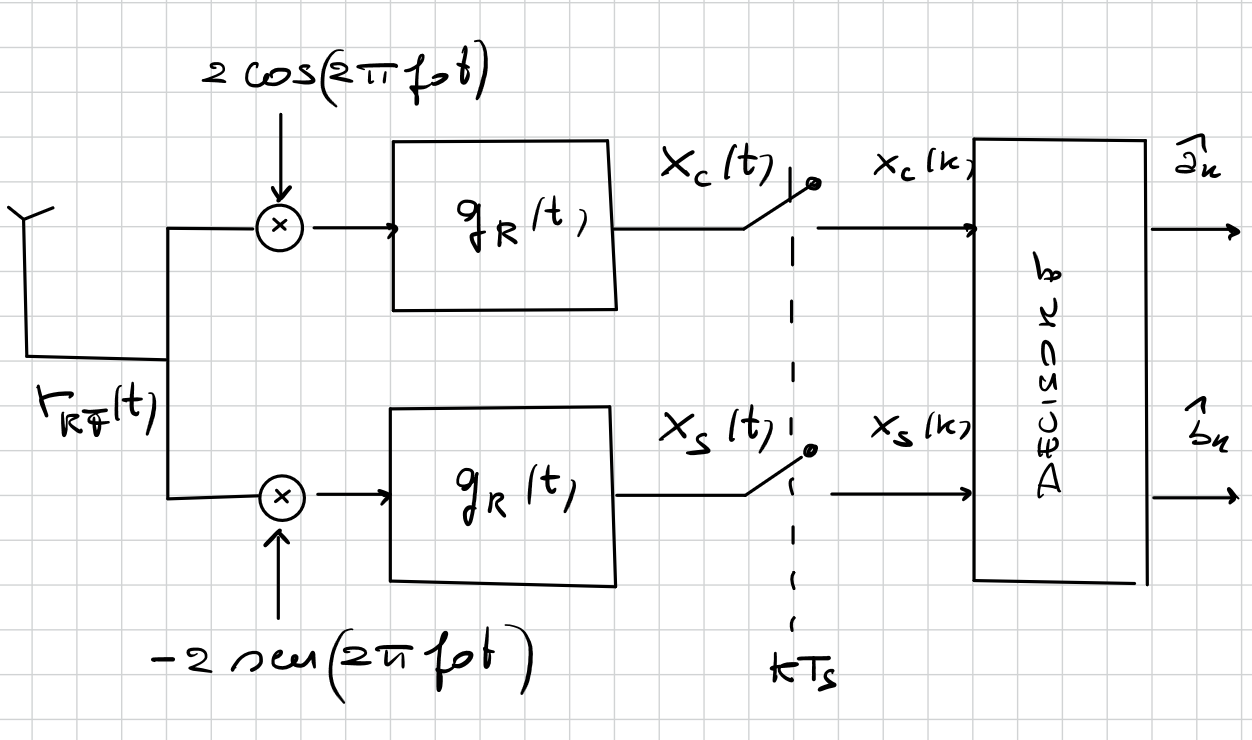
\includegraphics[scale=0.25]{../figures/qam_recv.png}
\end{center}

In questo caso prevediamo solo un'antenna a ricezione, che viene quindi sdoppiata e demodulata separatamente (nelle due fasi ortogonali seno/coseno). Quindi si campiona: un eventuale demapper prenderà entrambi i segnali $\hat{a}_k$ e $\hat{b}_k$ ricostruiti (i 2 canali ortogonali della QAM). 

Il segnale ricevuto sarà:
$$
r_{RF}(t) = S_{RF}(t) + W_{RF}(t)
$$
dove $S_{RF}$ comprende entrambi i canali ($x_C(t)$ e $x_S(t)$) mentre $W_{RF}$ è il rumore.
Da questo si ricavano entrambi i segnali come:
$$
\begin{cases}
	x_C(t) = r_{RF}(t) \, 2 \cos(2 \pi f_0 t) \circledast g_R(t) \\
	x_S(t) = - r_{RF}(t) \, 2 \sin(2 \pi f_0 t) \circledast g_R(t) \\
\end{cases}
$$

Prendiamo ad esempio uno solo dei due segnali, cioè il primo:
$$
x_C(t) = r_{RF}(t) \, 2 \cos(2 \pi f_0 t) \circledast g_R(t)
$$
$$
= 2 \left( I(t) \cos(2 \pi f_0 t) - Q(t) \sin(2 \pi f_0 t) \cos(2 \pi f_0 t) \circledast g_R(t) \right) + W_{RF}(t) 2 \cos (2 \pi f_0 t) \circledast g_R(t)
$$
dove il rumore va come $N_0 |G_R(f)|^2$ (e quindi $N_0$, come nel banda passante PAM).

Campionato periodo $T_S$, di questo rimane solo l'$a_i$ dall'$I(t)$:
$$
x_C(t) = \sum_i a_i g(t - i T_S) + n_C(t), \quad n_C \sim N_C = | G_R(f) |^2
$$
Il termine in $Q(t)$ svanisce in quanto viene campionato $T_S$. Prendiamolo separatamente:
$$
2 Q(t) \sin (2 \pi f_0 t) \cos (2 \pi f_0 t) \circledast g_R(t) = Q(t) \sin(4 \pi f_0 t)
$$
che campionato $\frac{1}{T_S}$ svanisce. In altre parole, il termine in quadratura, modulato in quadratura e demodulato non in quadratura, viene "modulato" 2 volte e svanisce alla frequenza di campionamento.

Da questo segue immediatamente anche il ramo in quadratura:
$$
\begin{cases}
	x_C(t) = \sum_i a_i g(t - i T_S) + n_C(t), \quad n_C \sim N_C \sim | G_R(f) |^2 \\
	x_S(t) = \sum_i b_i g(t - i T_S) + n_S(t), \quad n_S \sim N_S \sim | G_R(f) |^2
\end{cases}
$$

Notiamo che la densità spettrale di potenza dei rumori su entrambi i rami è la stessa.

Sempre dal punto di vista matematico, ci conviene riportare i due segnali in un unico segnale complesso (equivalente al corrispondente PAM):
$$
\begin{cases}
	x_C(k) = X_C(t = k T_S) = \sum_m a_{k - m} g(m T_S) + n_C(k) \\
	x_S(k) = X_S(t = k T_S) = \sum_m b_{k - m} g(m T_S) + n_S(k) 
\end{cases}
$$
da cui si ricava:
$$
x(k) = x_C(k) + j x_S(k) = \sum_m c_{k - m} g(m T_S) + n(k) 
$$
dove $n(k)$ va come il doppio di $n_C(k) = n_S(k)$, ovvero ha varianza:
$$
n(k) \sim \mathcal{N}_C(0, 2 N_0 |G_R(f)|^2)
$$

Come nel PAM, dobbiamo riscalare il segnale per ritrovare gli $a_k$, $b_k$:
$$
z(k) = \frac{x(k)}{\sqrt{\beta} g(0)} = c_k + n'(k)
$$
dove il nuovo trovato rumore avrà:
$$
n'(k) \sim \mathcal{N}_C \left( 0, \frac{2 N_0}{\beta} \right)
$$

\subsubsection{Probabilità di errore}

Abbiamo quindi racimolato abbastanza informazioni per iniziare la stima della probabilità di errore. Prendiamo una 4-QAM, per cui si hanno i soli 4 simboli trasmissibili:
$$
(1, j), \ (1, -j), \ (-1, j), \ (-1, -j)
$$

In tal caso la probabilità di errore è definita come:
$$
P(e) = \sum_{l = 1}^M P(e | c_k = c^{(l)}) P(c_k = c^{l}) = \frac{1}{4} \sum_{l = 1}^M P(e | c_k = c^{(l)})
$$
Restano da calcolare le $4$ probabilità di errore (relative ad ogni simbolo).

La prima cosa da fare è definire la strategia di decisione: per una 4-QAM adottiamo una decodifica bang-bang dove ci interessa solo il quadrante in cui ci troviamo (ovvero $x_C(k)$ e $x_S(k)$ minori/maggiori di zero). Per cui:
$$
P(e | c_k = c^{(l)}) = 1 - P( \neg e | c_K = c^{(l)} ), \quad
P( \neg e |  c_K = c^{(l)} ) = P( x_C(k) \geq 0, \, x_S(k) \geq 0 | c_k = c^{(l)})
$$
$$
= P(x_C(k) \geq 0 | a_k = a_k^{(l)}) P(x_S(k) \geq 0 | b_k = b_k^{(l)})
$$
Queste variabili sono indipendenti perché i rumori sono guassiani (ed indipendenti).
Quindi, svolgendo il calcolo, si ha dalla simmetria dei rumori: 
$$
= Q\left( -\frac{1}{\sigma_{n_C}} \right) Q\left( -\frac{1}{\sigma_{n_S}} \right) = Q^2 \left( - \frac{1}{\sigma_{n_C}} \right)^2
$$

Per cui ci si riporta a: 
$$
P(e | c_k = c^{(l)}) = 1 - Q\left( -\frac{1}{\sigma_{n_C}} \right)^2 = 1 - \left( 1 - Q \left( \frac{1}{\sigma_{n_C}} \right) \right)
$$
$$
\dots
$$
$$
= 2 Q\left( \frac{1}{\sigma_{n_C}} \right) - Q^2 \left( \frac{1}{\sigma_{n_C}} \right) \approx 2 Q \left( \frac{1}{\sigma_{n_C}} \right)
$$
risparmiando fastidiosi calcoli, ovvero il doppio della probabilità di errore dell'equivalente PAM. Alternativamente questo può intendersi come:
$$
P(e | c_k = c^{(l)}) = P(A) + P(B) - P(A \cap B) = 1 - Q \left( - \frac{1}{\sigma_{n_C}} \right) + Q \left( \frac{1}{\sigma_{n_C}} \right) - Q^2 \left( \frac{1}{\sigma_{n_C}} \right)
$$

\par\smallskip

A questo punto possiamo riportarci alle definizioni su energia e potenza, con:
$$
P(e) \approx 2 Q \left( \sqrt{\frac{\beta}{N_0}} \right) = 2 Q \left( \sqrt{\frac{6}{M - 1}\frac{E_r}{N_0}} \right)
$$
e via dicendo, in maniera analoga alla PAM.



\end{document}
